\documentclass{xjtureport}
\usepackage[linesnumbered,ruled]{algorithm2e}
% =============================================
% Part 0 Edit the info
% =============================================

\major{计算机科学与技术}
\name{曾锦程}
\title{软件定义网络实验报告}
\stuid{2203613040}
\college{计算机学院}
\date{\zhtoday}
\lab{Personal Device}
\course{软件定义网络}
\instructor{张鹏}
\grades{}
\expname{Lab1 Fattree}
\exptype{}
\partner{}

\begin{document}
% =============================================
% Part 1 Header
% =============================================
\makecover
\makeheader

% =============================================
% Part 2 Main document
% =============================================

\section{实验目的和要求}
(1)使用 Mininet 的Python API搭建 k=4 的 fat tree 拓扑;\par
(2)使用 pingall 查看各主机之间的连通情况;\par
(3)若主机之间未连通,分析原因并解决(使用 wireshark 抓包分析)\par
(4)若主机连通,分析数据包的路径(提示: ovs-appctl fdb/show 查看MAC表)\par
(5)完成实验报告并提交到思源学堂\par
(6)要求不能使用控制\par
\section{实验内容和步骤}
–编写Fattree.py,使用python接口来搭建Fattree网络\par
–使用\texttt{pingall}指令,测试网络是否ping通\par
–使用Wireshark抓包分析网络\par
\section{实验环境}
虚拟机Virtual Box,Mininet,OVS,Wireshark。
\section{实验原理分析}
\subsection{Fattree介绍}
Fattree是一种网络拓扑结构,它被广泛应用于数据中心网络中,可以提供高带宽、低延迟、可扩展的网络连接。Fattree拓扑结构由多个层级组成,每个层级由多个交换机组成,交换机之间通过链路连接。Fattree拓扑结构包含三个层级:边缘层(edge layer)、聚合层(aggregation layer)和核心层(core layer)。\par
在Fattree拓扑结构中,边缘层连接着数据中心的端口,聚合层提供了高速的连接,同时在核心层通过最短路径提供最快速的转发速度。在Fattree拓扑结构中,每个交换机的端口数量相同,交换机的规模是固定的,因此它具有可扩展性和高度的容错性。\par
Fattree拓扑结构的优点在于,它可以提供非阻塞的带宽和低延迟的网络连接,同时具有可扩展性和容错性。它适用于大型数据中心,特别是那些需要高性能和高可用性的应用程序,如云计算、大数据和机器学习等。\par
\subsection{拓扑图分析} 
\begin{figure}[H]
	\centering
	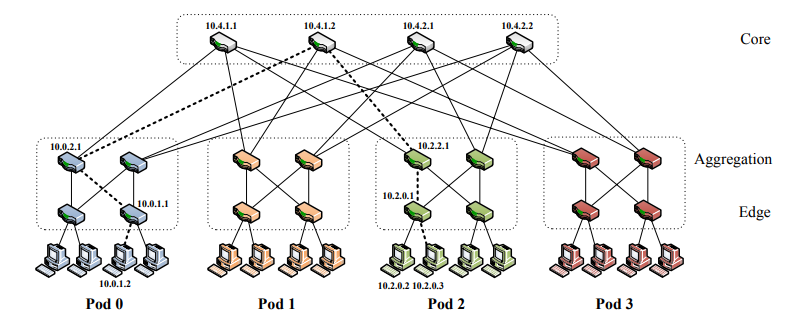
\includegraphics[width=0.8\linewidth]{fattree topo.png}
	\caption{Fattree(k=4)}
\end{figure}
\subsubsection{节点个数分析}
(i) Core Switch的个数为:$k^2 \over 4$\par
(ii) Pod数量为$k$个\par
(iii)每个Pod中含有Aggregation Switch个数为$k \over 2$\par
(iv)每个Pod中含有Edge Switch个数为$k \over 2$\par 
(v)每个Pod中含有的Host个数为$k^2 \over 4$
\subsubsection{路由分析}
(i)对于Core层与Aggregation层分析如下:\par
\quad \quad 对于每个Core Switch,需要和$k/2$个Aggregation Switch连接,而连接的Aggregation的编号在每个Pod中相同,编号计算方法为:
$$ AggregationNumber = CoreNumber // (k/2)$$
\quad \quad(ii)对于Aggregation层与Edge层分析如下:\par 
\quad \quad 对于每个Aggregation Switch都需要和本Pod中的每个Edge Switch连接。\par
(iii)对于Edge层与Host层分析如下:\par 
\quad \quad 对于每个Pod中的Edge Switch都需要负责连接本Pod中的$k/2$个Host,Host的编号计算方法为:
$$ HostNumber_{Begin} = EdgeNumber*(k/2) $$
$$ HostNumber_{End} = EdgeNumber*(k/2) + k/2 - 1$$
\subsection{工具介绍}
\subsubsection{Mininet}
Mininet是一个用于网络仿真的开源工具,它能够模拟一个包括多个主机、交换机、路由器等网络设备的虚拟网络。使用Mininet,用户可以在自己的计算机上快速搭建一个网络环境,进行网络应用的测试、开发和教学等工作。

Mininet的虚拟网络是基于Linux内核实现的,并且使用Open vSwitch作为虚拟交换机。它提供了丰富的API和命令行工具,使得用户可以方便地创建、配置和控制虚拟网络。用户可以在虚拟网络中安装各种网络应用程序,如路由协议、拥塞控制算法、数据中心网络等,并进行测试和评估。

Mininet还提供了一些方便的工具和库,如网络拓扑生成器、流量发生器、OpenFlow控制器等,使得用户可以快速地搭建不同类型的虚拟网络,并进行灵活的网络测试和研究。

Mininet的优点在于它具有开源、灵活、易用等特点,可以在本地环境中快速构建网络实验室,节省了实验成本和时间。因此,Mininet被广泛应用于网络教育、网络研究和网络应用开发等领域。
\subsubsection{OVS}
OVS(Open vSwitch)是一款开源的软件交换机,它提供了多种网络虚拟化技术和高级网络功能,如流量控制、负载均衡、网络隔离和安全等。OVS可以用于虚拟化环境、数据中心网络、云计算和SDN(软件定义网络)等场景。

OVS的核心是一个模块化的软件交换机,它可以在Linux内核中作为一个内核模块运行。OVS还提供了一个用户空间的管理工具(ovs-vsctl),用于管理OVS交换机的配置和运行状态。OVS支持多种数据平面,如Linux内核数据平面、DPDK(Data Plane Development Kit)数据平面和NetFlow数据平面等,可以根据需求选择适合的数据平面。

OVS支持多种网络虚拟化技术,如VLAN、VXLAN、GRE、Geneve等,可以在虚拟网络中实现多租户隔离和跨物理网络的互联。OVS还支持OpenFlow协议,可以通过OpenFlow控制器实现SDN网络控制和编程。OVS还提供了多种高级网络功能,如流量镜像、流量过滤、QoS(Quality of Service)和负载均衡等,使得网络管理更加灵活和高效。

总之,OVS是一款功能强大、灵活可扩展的软件交换机,它提供了多种网络虚拟化技术和高级网络功能,可以满足不同场景下的网络需求。
\section{实验过程}
\subsection{使用python API来构建fattree}
本实验要求为搭建k=4的fattree,实际上做了上述对fattree的拓扑分析后,可以发现很容易就做出k=n的fattree,于是将代码扩充成符合k为任意符合条件值的fattree。(完整代码见附录)
\begin{figure}[H]
	\centering
	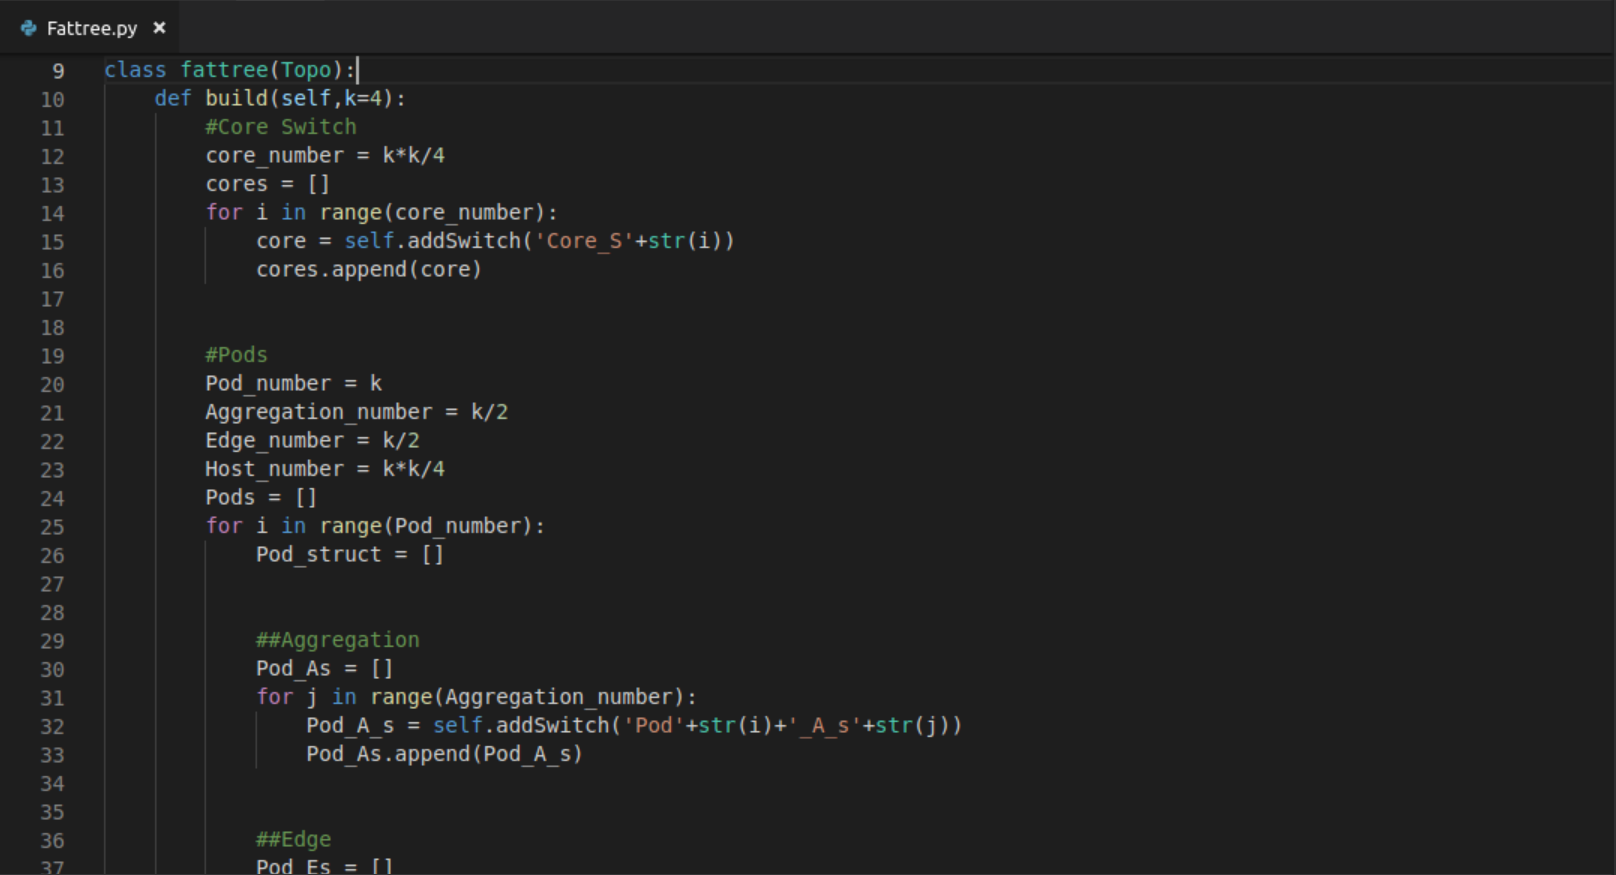
\includegraphics[width=0.6\linewidth]{code.png}
	\caption{代码片段}
\end{figure}
\begin{figure}[H]
	\centering
	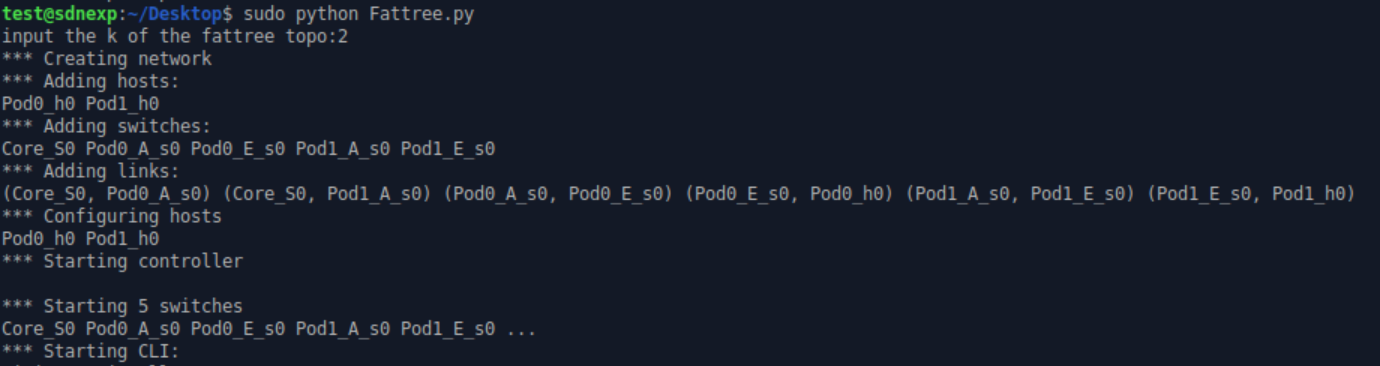
\includegraphics[width=0.6\linewidth]{k2.png}
	\caption{Fattree(k=2)}
\end{figure}
\begin{figure}[H]
	\centering
	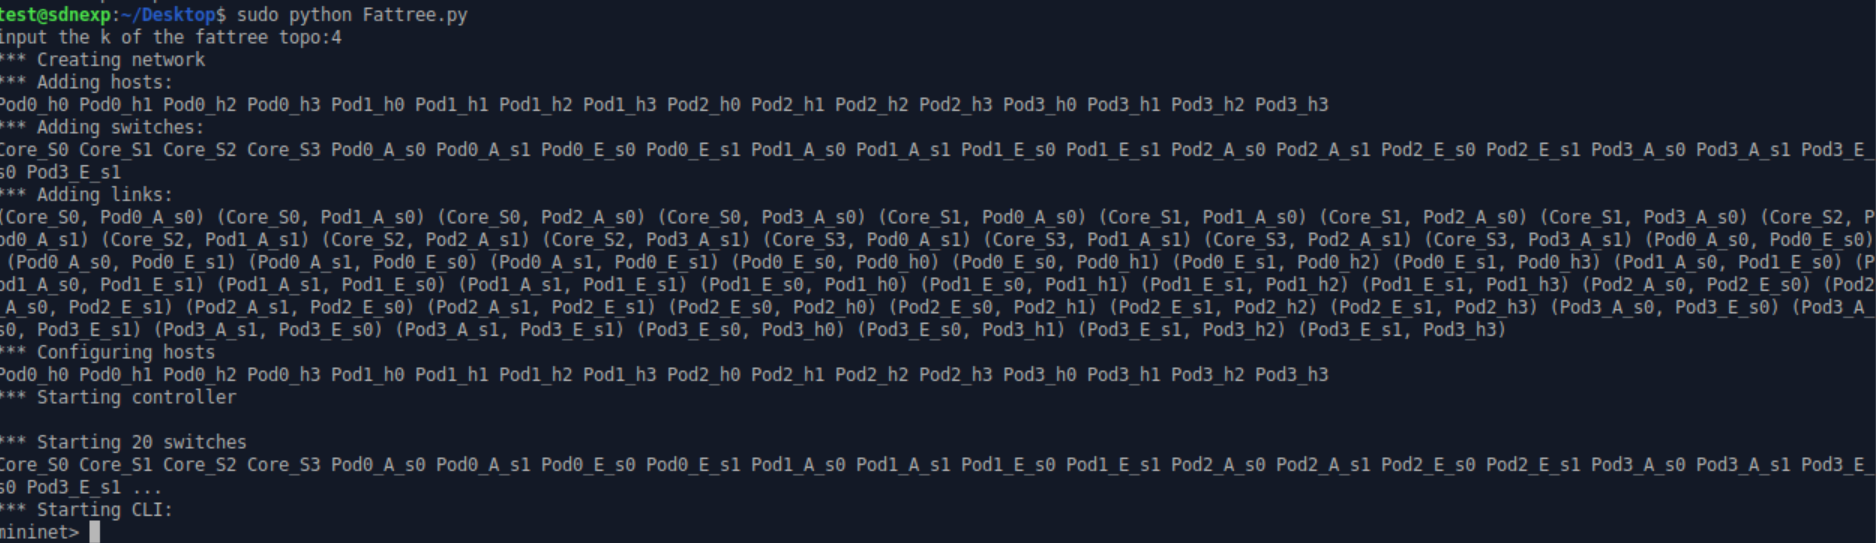
\includegraphics[width=0.6\linewidth]{k4.png}
	\caption{Fattree(k=4)}
\end{figure}
\begin{figure}[H]
	\centering
	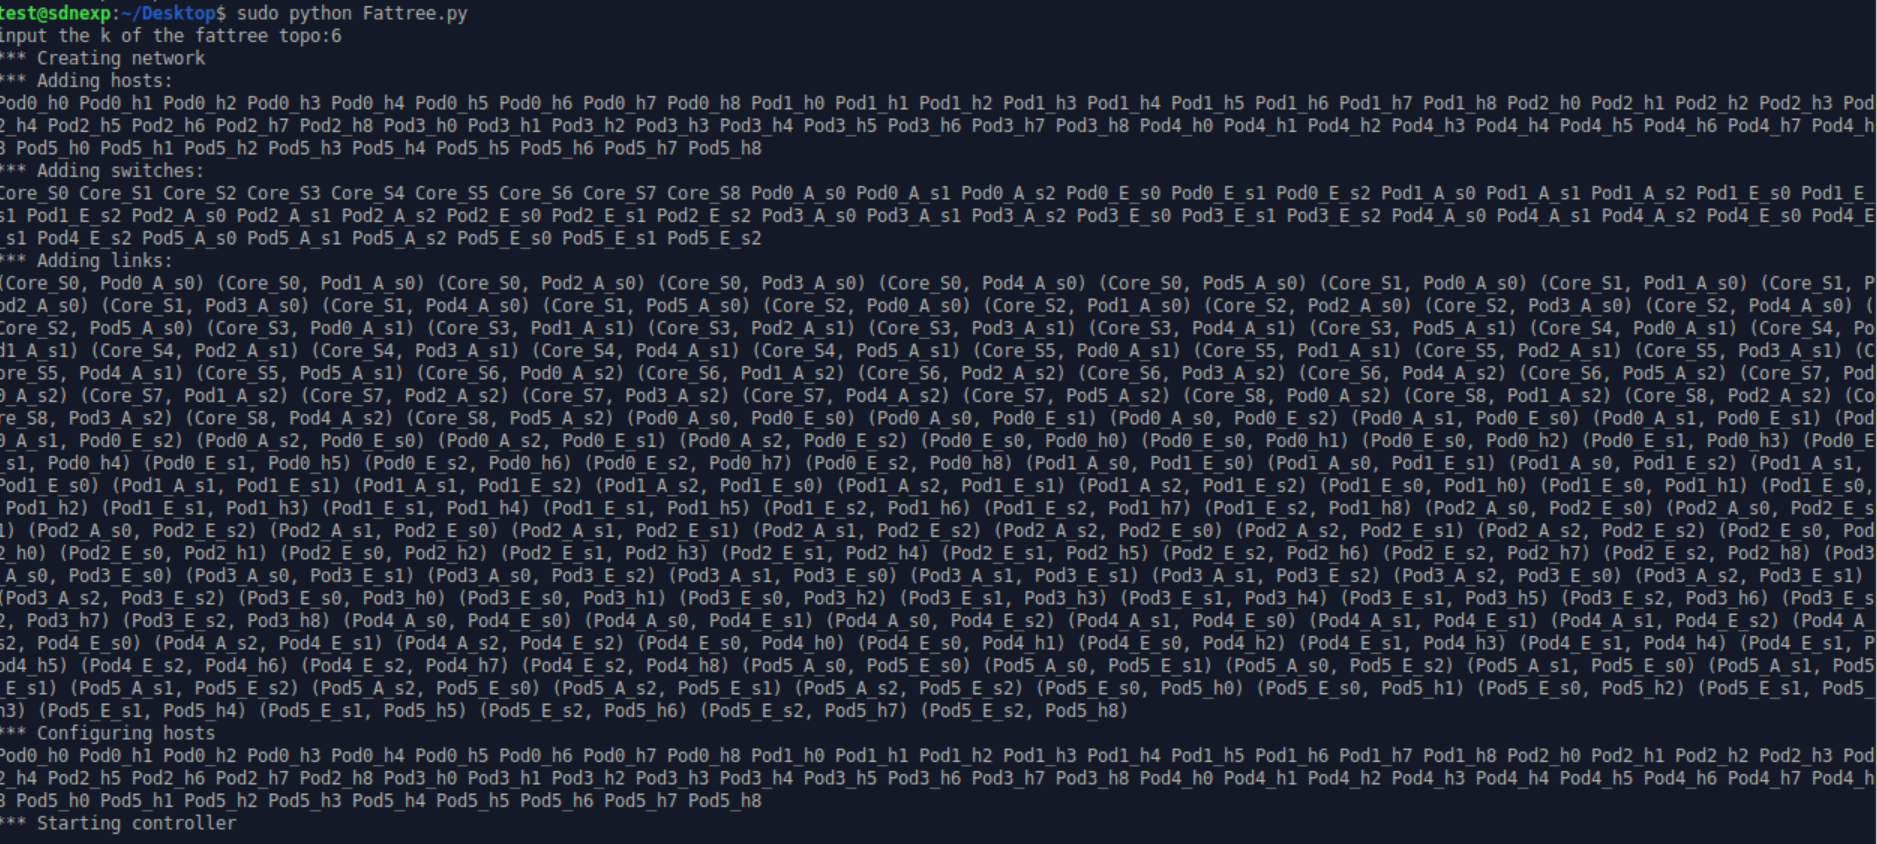
\includegraphics[width=0.6\linewidth]{k6.png}
	\caption{Fattree(k=6)}
\end{figure}
\subsection{使用python来调用命令行,实现给每个路由器配置STP协议}
之前没有配置,导致pingall unreachable,对使用xterm指令,打开h0,让其ping 10.2,并在h0进行抓包分析。
\begin{figure}[H]
	\centering
	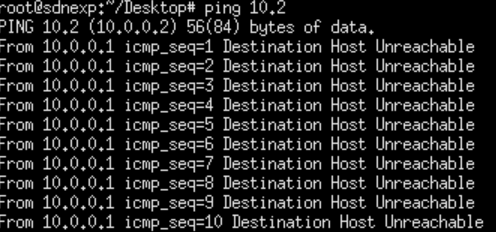
\includegraphics[width=0.6\linewidth]{ping.png}
	\caption{h0 ping 10.2}
\end{figure}
\begin{figure}[H]
	\centering
	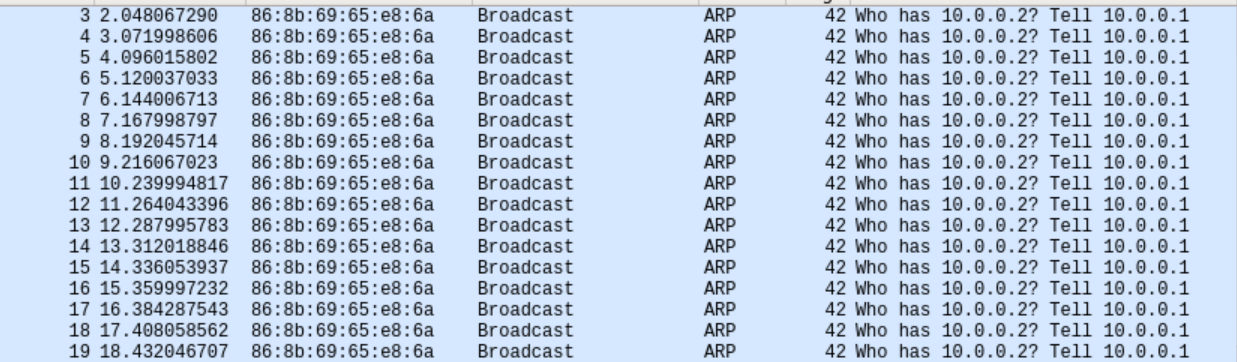
\includegraphics[width=0.6\linewidth]{wire.png}
	\caption{h0 wireshark}
\end{figure}
发现在ping的过程中,主机一直在广播ARP包,但是没有网关的回应,说明是STP协议未配置,路由器并没有学习到拓扑结构,所以无法应答ARP,加入以下代码,让其自动给每个路由器配置STP协议,再观察结果。
\begin{lstlisting}[language=Python]
for i in range(core_number): 
	os.system('sudo ovs-vsctl set bridge '+'Core_s'+str(i)+' stp_enable=true')
	os.system('sudo ovs-vsctl del-fail-mode '+'Core_s'+str(i))
for i in range(Pod_number):
	for j in range(Aggregation_number):
		os.system('sudo ovs-vsctl set bridge '+'Pod'+str(i)+'_A_s'+str(j)+' stp_enable=true')
		os.system('sudo ovs-vsctl del-fail-mode '+'Pod'+str(i)+'_A_s'+str(j))
	for j in range(Edge_number):
		os.system('sudo ovs-vsctl set bridge '+'Pod'+str(i)+'_E_s'+str(j)+' stp_enable=true')
		os.system('sudo ovs-vsctl del-fail-mode '+'Pod'+str(i)+'_E_s'+str(j))
\end{lstlisting}
\quad \quad 使用命令pingall,发现成功ping通所有路径。
\begin{figure}[H]
	\centering
	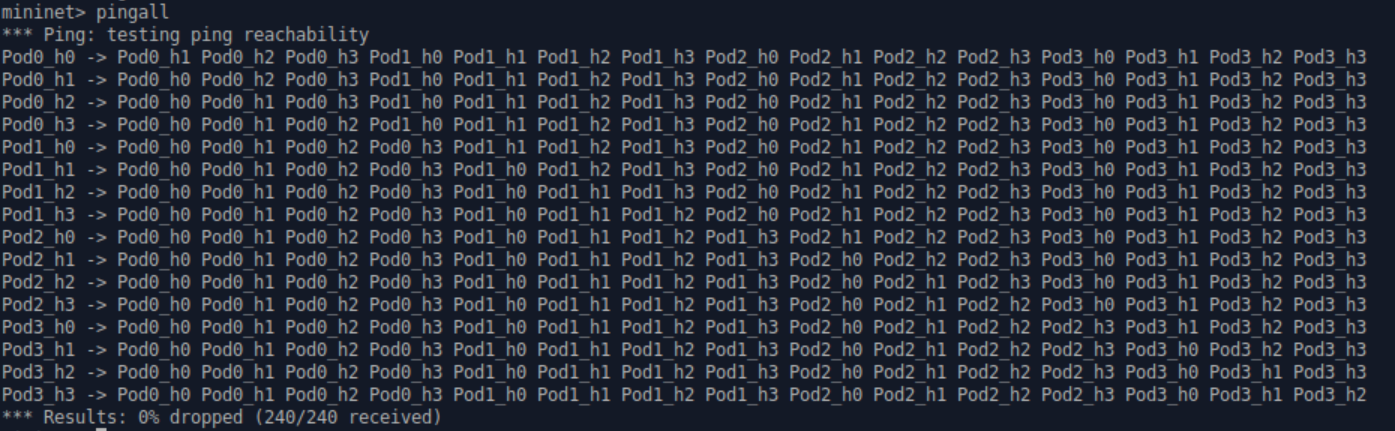
\includegraphics[width=0.6\linewidth]{pingall.png}
	\caption{pingall}
\end{figure}
\begin{figure}[H]
	\centering
	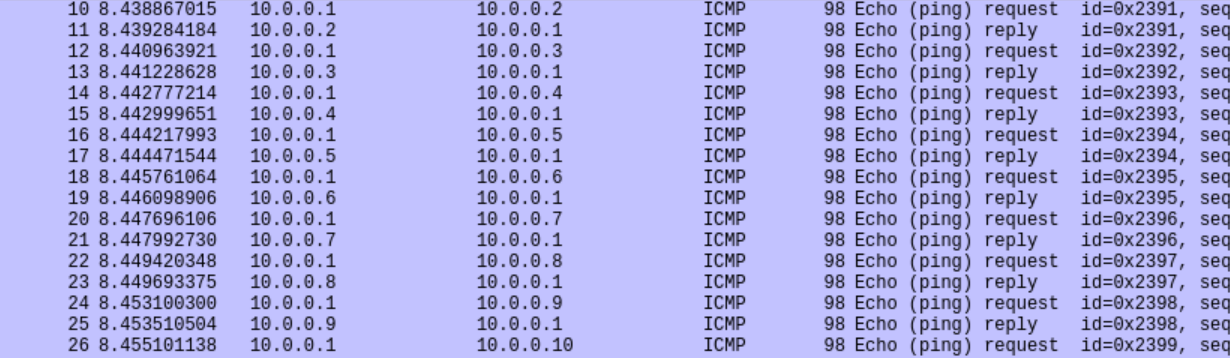
\includegraphics[width=0.6\linewidth]{pingallwire.png}
	\caption{wireshark}
\end{figure}
同时打开主机h0,ping 10.16,发现ping通,而且抓包分析可以看出,主机发送ARP包,成功获得了交换机的应答!
\begin{figure}[H]
	\centering
	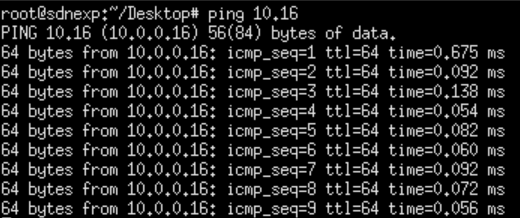
\includegraphics[width=0.6\linewidth]{ping1.png}
	\caption{h0 ping 10.16}
\end{figure}
\begin{figure}[H]
	\centering
	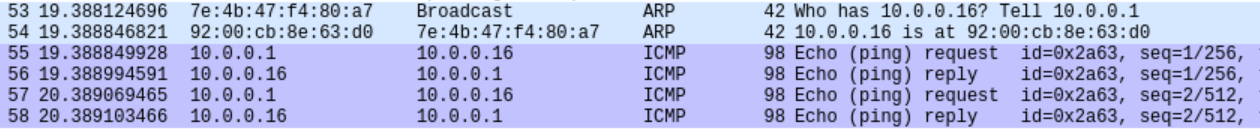
\includegraphics[width=0.6\linewidth]{wire1.png}
	\caption{h0 wireshark}
\end{figure}
\subsection{分析数据包的路径}
先使用\texttt{xx ifconfig}指令查看主机的mac地址:
\begin{figure}[H]
	\centering
	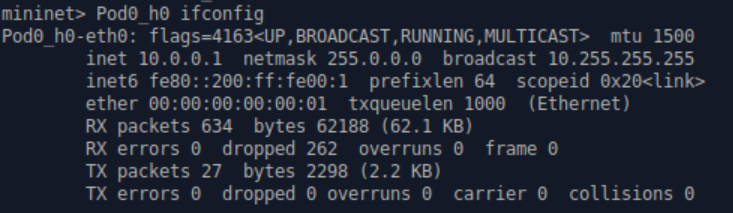
\includegraphics[width=0.6\linewidth]{h0.png}
	\caption{h0 ifconfig}
\end{figure}
\begin{figure}[H]
	\centering
	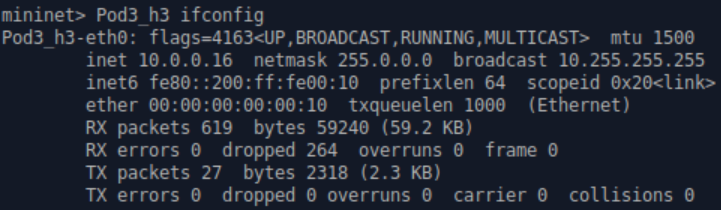
\includegraphics[width=0.6\linewidth]{h15.png}
	\caption{h15 ifconfig}
\end{figure}
可以看出h0的mac地址为00:01,h15的mac地址为00:10,现以h0向h15ping,分析该数据包的路径,查看所有交换机的Mac表(调用Macshow.py,见附录)。
\begin{figure}[H]
	\centering
	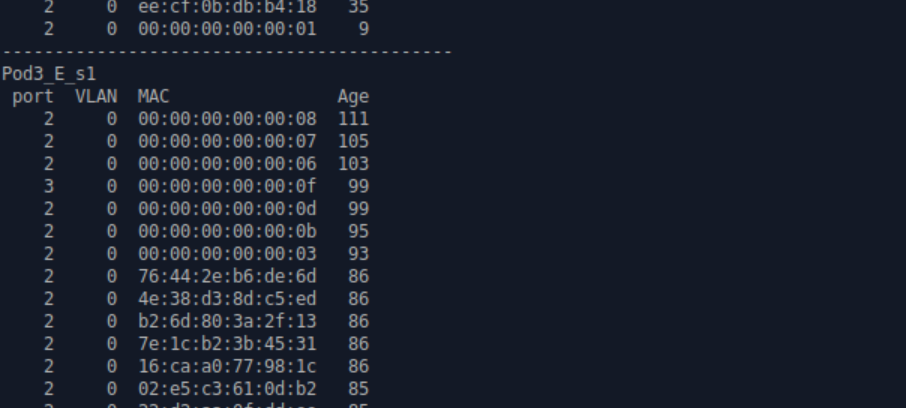
\includegraphics[width=0.6\linewidth]{macshow.png}
	\caption{mac show实例}
\end{figure}
\section{实验结果分析}
\subsection{分析数据包的路径}
查阅所有交换机的mac表,只要同时包含00:01和00:10两项,说明数据包通过该交换机,于是可以得出下表:
\begin{table}[H]
	\begin{center}
		\begin{tabular}{lllllllll}
			\toprule
			Hop & Hop-1 & Hop-2 & Hop-3 & Hop-1 & Hop-2 & Hop-3 & Hop-4  \\
			\midrule
			00:01->00:10  & h0 & Pod0-E-s0 & Pod0-A-s1 & Core-s3 & Pod3-A-s1 & Pod3-E-s1 & h15  \\
			\bottomrule
		\end{tabular}
	\end{center}
	\caption{数据包传输路径表}
\end{table}
\begin{figure}[H]
	\centering
	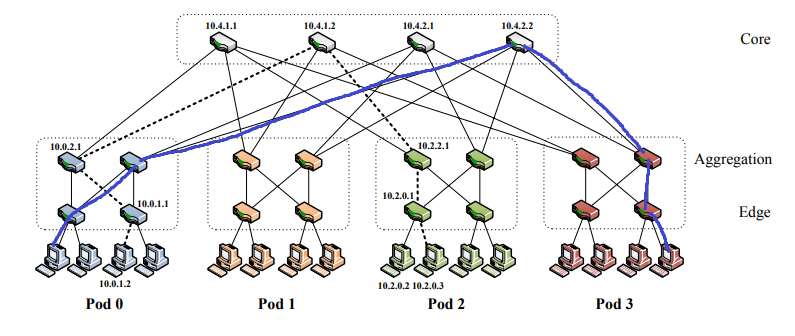
\includegraphics[width=0.8\linewidth]{fattree topo1.png}
	\caption{数据包传输路径图}
\end{figure}
其中Edge层与主机层路径和主机编号有关,Aggregation层与Edge层路径和Edge switch所连主机有关,Core与Aggregation层路径和Core Switch编号有关。
\section{实验感悟}
(1)基本了解了在linux系统调用mininet的命令,以及一些基本shell命令的调用\par
(2)对Fattree拓扑结构有了更深的理解\par
(3)学会了通过查看路由器MAC表来分析数据包路径的方法\par
(4)学会了Python面对对象构建网络拓扑的方法,学会了如何在python中调用命令行,对python有了更深的理解。
\section{附录}
Fattree.py
\begin{lstlisting}[language=Python]
from mininet.topo import Topo
from mininet.net import Mininet
from mininet.cli import CLI
from mininet.log import setLogLevel
import os
import commands


class fattree(Topo):
	def build(self,k=4):
		#Core Switch
		core_number = k*k/4
		cores = []
		for i in range(core_number):
			core = self.addSwitch('Core_s'+str(i))
			cores.append(core)


		#Pods
		Pod_number = k
		Aggregation_number = k/2
		Edge_number = k/2
		Host_number = k*k/4
		Pods = []
		for i in range(Pod_number):
			Pod_struct = []


			##Aggregation
			Pod_As = []
			for j in range(Aggregation_number):
				Pod_A_s = self.addSwitch('Pod'+str(i)+'_A_s'+str(j))
				Pod_As.append(Pod_A_s)


			##Edge
			Pod_Es = []
			for j in range(Edge_number):
				Pod_E_s = self.addSwitch('Pod'+str(i)+'_E_s'+str(j))
				Pod_Es.append(Pod_E_s)


			##Host
			Pod_Hs = []
			for j in range(Host_number):
				Pod_H = self.addHost('Pod'+str(i)+'_h'+str(j))
				Pod_Hs.append(Pod_H)
				Pod_struct.append(Pod_As)
				Pod_struct.append(Pod_Es)
				Pod_struct.append(Pod_Hs)
				Pods.append(Pod_struct)


		#Core Link
		for i in range(len(cores)):
			a_number = i//(k/2)
			for j in range(len(Pods)):
			self.addLink(cores[i],Pods[j][0][a_number])


		#Pod Switch Link
		for i in range(len(Pods)):
			for j in range(len(Pods[0][0])):
				for k in range(len(Pods[0][1])):
					self.addLink(Pods[i][0][j],Pods[i][1][k])


		#Host Link
		Host_number = Pod_number
		for i in range(len(Pods)):
			for j in range(len(Pods[0][1])):
				h_number = j*Host_number/2
				for k in range(Host_number/2):
					self.addLink(Pods[i][1][j],Pods[i][2][k+h_number])



def run(k=4):
	topo = fattree(k)
	net = Mininet(topo,controller=None)
	core_number = k*k/4
	Pod_number = k
	Aggregation_number = k/2
	Edge_number = k/2
	Host_number = k
	for i in range(core_number): 
		os.system('sudo ovs-vsctl set bridge '+'Core_s'+str(i)+' stp_enable=true')
		os.system('sudo ovs-vsctl del-fail-mode '+'Core_s'+str(i))
	for i in range(Pod_number):
		for j in range(Aggregation_number):
			os.system('sudo ovs-vsctl set bridge '+'Pod'+str(i)+'_A_s'+str(j)+' stp_enable=true')
			os.system('sudo ovs-vsctl del-fail-mode '+'Pod'+str(i)+'_A_s'+str(j))
		for j in range(Edge_number):
			os.system('sudo ovs-vsctl set bridge '+'Pod'+str(i)+'_E_s'+str(j)+' stp_enable=true')
			os.system('sudo ovs-vsctl del-fail-mode '+'Pod'+str(i)+'_E_s'+str(j))

	net.start()
	CLI(net)
	net.stop()


if __name__ == '__main__':
	k = int(input('input the k of the fattree topo:'))
	setLogLevel('info')
	run(k)
\end{lstlisting}
\quad \quad Macshow.py
\begin{lstlisting}[language=Python]
import os
import commands

def macshow(k=4):
	core_number = k*k/4
	Pod_number = k
	Aggregation_number = k/2
	Edge_number = k/2
	for i in range(core_number): 
		print('-------------------------------------------')
		print('Core_s'+str(i))
		os.system('sudo ovs-appctl fdb/show '+'Core_s'+str(i))
	for i in range(Pod_number):
		for j in range(Aggregation_number):
			print('-------------------------------------------')
			print('Pod'+str(i)+'_A_s'+str(j))
			os.system('sudo ovs-appctl fdb/show '+'Pod'+str(i)+'_A_s'+str(j))
		for j in range(Edge_number):
			print('-------------------------------------------')
			print('Pod'+str(i)+'_E_s'+str(j))
			os.system('sudo ovs-appctl fdb/show '+'Pod'+str(i)+'_E_s'+str(j))


if __name__ == '__main__':
	k = int(input('input the k of the fattree topo:'))
	macshow(k)
\end{lstlisting}
\end{document}
